\documentclass[11pt,addpoints,answers]{exam}
\usepackage[margin=1in]{geometry}
\usepackage{amsmath, amsfonts}
\usepackage{enumerate}
\usepackage{graphicx}
\usepackage{titling}
\usepackage{url}
\usepackage{xfrac}
\usepackage{geometry}
\usepackage{graphicx}
\usepackage{natbib}
\usepackage{amsmath}
\usepackage{amssymb}
\usepackage{amsthm}
\usepackage{paralist}
\usepackage{epstopdf}
\usepackage{tabularx}
\usepackage{longtable}
\usepackage{multirow}
\usepackage{multicol}
\usepackage[colorlinks=true,urlcolor=blue]{hyperref}
\usepackage{fancyvrb}
\usepackage{algorithm}
\usepackage{algorithmic}
\usepackage{float}
\usepackage{paralist}
\usepackage[svgname]{xcolor}
\usepackage{enumerate}
\usepackage{array}
\usepackage{times}
\usepackage{url}
\usepackage{comment}
\usepackage{environ}
\usepackage{times}
\usepackage{textcomp}
\usepackage{caption}
\usepackage[colorlinks=true,urlcolor=blue]{hyperref}
\usepackage{listings}
\usepackage{parskip} % For NIPS style paragraphs.
\usepackage[compact]{titlesec} % Less whitespace around titles
\usepackage[inline]{enumitem} % For inline enumerate* and itemize*
\usepackage{datetime}
\usepackage{comment}
% \usepackage{minted}
\usepackage{lastpage}
\usepackage{color}
\usepackage{xcolor}
\usepackage{listings}
\usepackage{tikz}
\usetikzlibrary{shapes,decorations,bayesnet}
%\usepackage{framed}
\usepackage{graphicx}
\usepackage{booktabs}
\usepackage{cprotect}
\usepackage{xcolor}
\usepackage{verbatimbox}
\usepackage[many]{tcolorbox}
\usepackage{cancel}
\usepackage{wasysym}
\usepackage{mdframed}
\usepackage{subcaption}
\usetikzlibrary{shapes.geometric}

size\newtcbtheorem[]{solution}{Solution}{breakable, fonttitle=\bfseries}{x}

\begin{document}
\begin{center}
    \textsc{\LARGE HW2-18-794: Introduction to Deep Learning and Pattern Recognition for Computer Vision} \\
    \vspace{1em}
    \textsc{\large Assignment 2: Face Detection} \\
    \vspace{0.5em}
    \textsc{\large Instructor: Marios Savvides} \\
    \vspace{0.5em}
    \textbf{Due Date:} Oct 19, 2023 \\
    \vspace{0.5em}
    \textbf{Total Points:} 100 \\
    \vspace{0.5em}
    \textbf{Submission:} Submit your solutions and plots on Gradescope.
\end{center}

\section*{START HERE: Instructions}
\begin{itemize}
\item \textbf{Collaboration policy:} All are encouraged to work together BUT you must do your own work (code and write up). If you work with someone, please include their name in your write-up and cite any code that has been discussed. If we find highly identical write-ups or code or lack of proper accreditation of collaborators, we will take action according to strict university policies. See the \href{hhttps://www.cmu.edu/policies/student-and-student-life/academic-integrity.html}{Academic Integrity Section} detailed in the initial lecture for more information.

\item\textbf{Late Submission Policy:} There are a \textbf{total of 5} late days across all homework submissions. Submissions more than 5 days after the deadline will receive a 0.

\textbf{For those students taking Mini-1 (semi-semester), you cannot submit it later than Oct 21, 2023, as the grading deadline of mini-1 is due on Oct 23, 2023.}

\item\textbf{Submitting your work:}

\begin{itemize}

\item We will be using Gradescope (\url{https://gradescope.com/}) to submit the Problem Sets. Please use the provided template only. Submissions must be written in LaTeX. All submissions not adhering to the template will not be graded and receive a zero. 
\item \textbf{Deliverables:} Please submit all the \texttt{.py} files. Add all relevant plots and text answers in the boxes provided in this file. TO include plots you can simply modify the already provided latex code. Submit the compiled \texttt{.pdf} report as well.
\end{itemize}
\end{itemize}
\emph{NOTE: Partial points will be given for implementing parts of the homework even if you don't get the mentioned numbers as long as you include partial results in this pdf.}
\clearpage

\section*{Overview}
In this assignment, you will train and test a state-of-the-art face detector that is deployed in the real world applications.

\section{Understand your data (POINTS : 30)}
Understanding your data is always the first step in training deep learning models, which
will greatly ease the following works. This step usually involves statistical analysis,
preprocessing, and visualization for detection datasets.

Data path: 

\url{https://drive.google.com/file/d/1799456S54_M7CS9Gom1xrD9_tIKavPuB/view?usp=sharing}

Note 1. The bounding box is indicated by the first 4 floats and is in (x1, y1, w, h). Where
x1, y1 is the top-left corner, followed by the 5 landmarks points ($L_x$, $L_y$), each landmark point 
 is followed by a 0/1 that you can ignore. The landmarks
might be -1 indicating no landmark available for this face.


\subsection{Write code to do the following statistical analysis}

1. Total number of ground truths (GT), i.e., faces, for training and validation.


2. Average area, width, and height of bounding boxes


3. Are faces uniformly distributed on images? Give your analysis.


4. Check if any GT exceeds the range of the image. If yes, how do you plan to solve it?


5. How serious is the mutual overlap among GTs? Calculate the percentage of GTs that overlap with one another (i.e., overlapped GT vs total number
of GT). Hint: check the overlap using IOU $>$ 0.

\begin{solution*}{}
Enter your solution here

For training data:

1. GT count:  159422

2. ave area:  3851.279020461417

ave w:  28.948482643549823

ave h:  37.398778085835076

3. No, average center value:

img center:  512.0 384.00535678442395

box center:  508.95301209353676 304.4233459203131

Also, with box center x and y location in plot:

\begin{figure}[H]
	\centering
	\includegraphics[width=0.8\linewidth]{img/1_tx.png}
\end{figure}

\begin{figure}[H]
	\centering
	\includegraphics[width=0.8\linewidth]{img/1_ty.png}
\end{figure}

We can see the values aren't the same and uniformly distributed.

4. No exceeding:

exceed h:  0

exceed w:  0

5. percentage of GTs:

Overlap:  0.12396657926760422



For val data:

1. GT count:  39707

2. ave area:  3834.9729266879895

ave w:  29.191981262749643

ave h:  37.60183342987383

3. No, average center value:

img center:  512.0 383.90033494509925

box center:  509.62418152513345 288.8188400322353

Also, with box center x and y location in plot:

\begin{figure}[H]
	\centering
	\includegraphics[width=0.8\linewidth]{img/1_vx.png}
\end{figure}

\begin{figure}[H]
	\centering
	\includegraphics[width=0.8\linewidth]{img/1_vy.png}
\end{figure}

We can see the values aren't the same and uniformly distributed.

4. No exceeding:

exceed h:  0

exceed w:  0

5. percentage of GTs:

Overlap:  0.12118769990178055


\end{solution*}

\subsection{Visualize the first 4 images and their ground truths, including the faces (in
green) and landmarks (in red).}


\begin{solution*}{}
Enter your solution here
\begin{figure}[H]
	\centering
	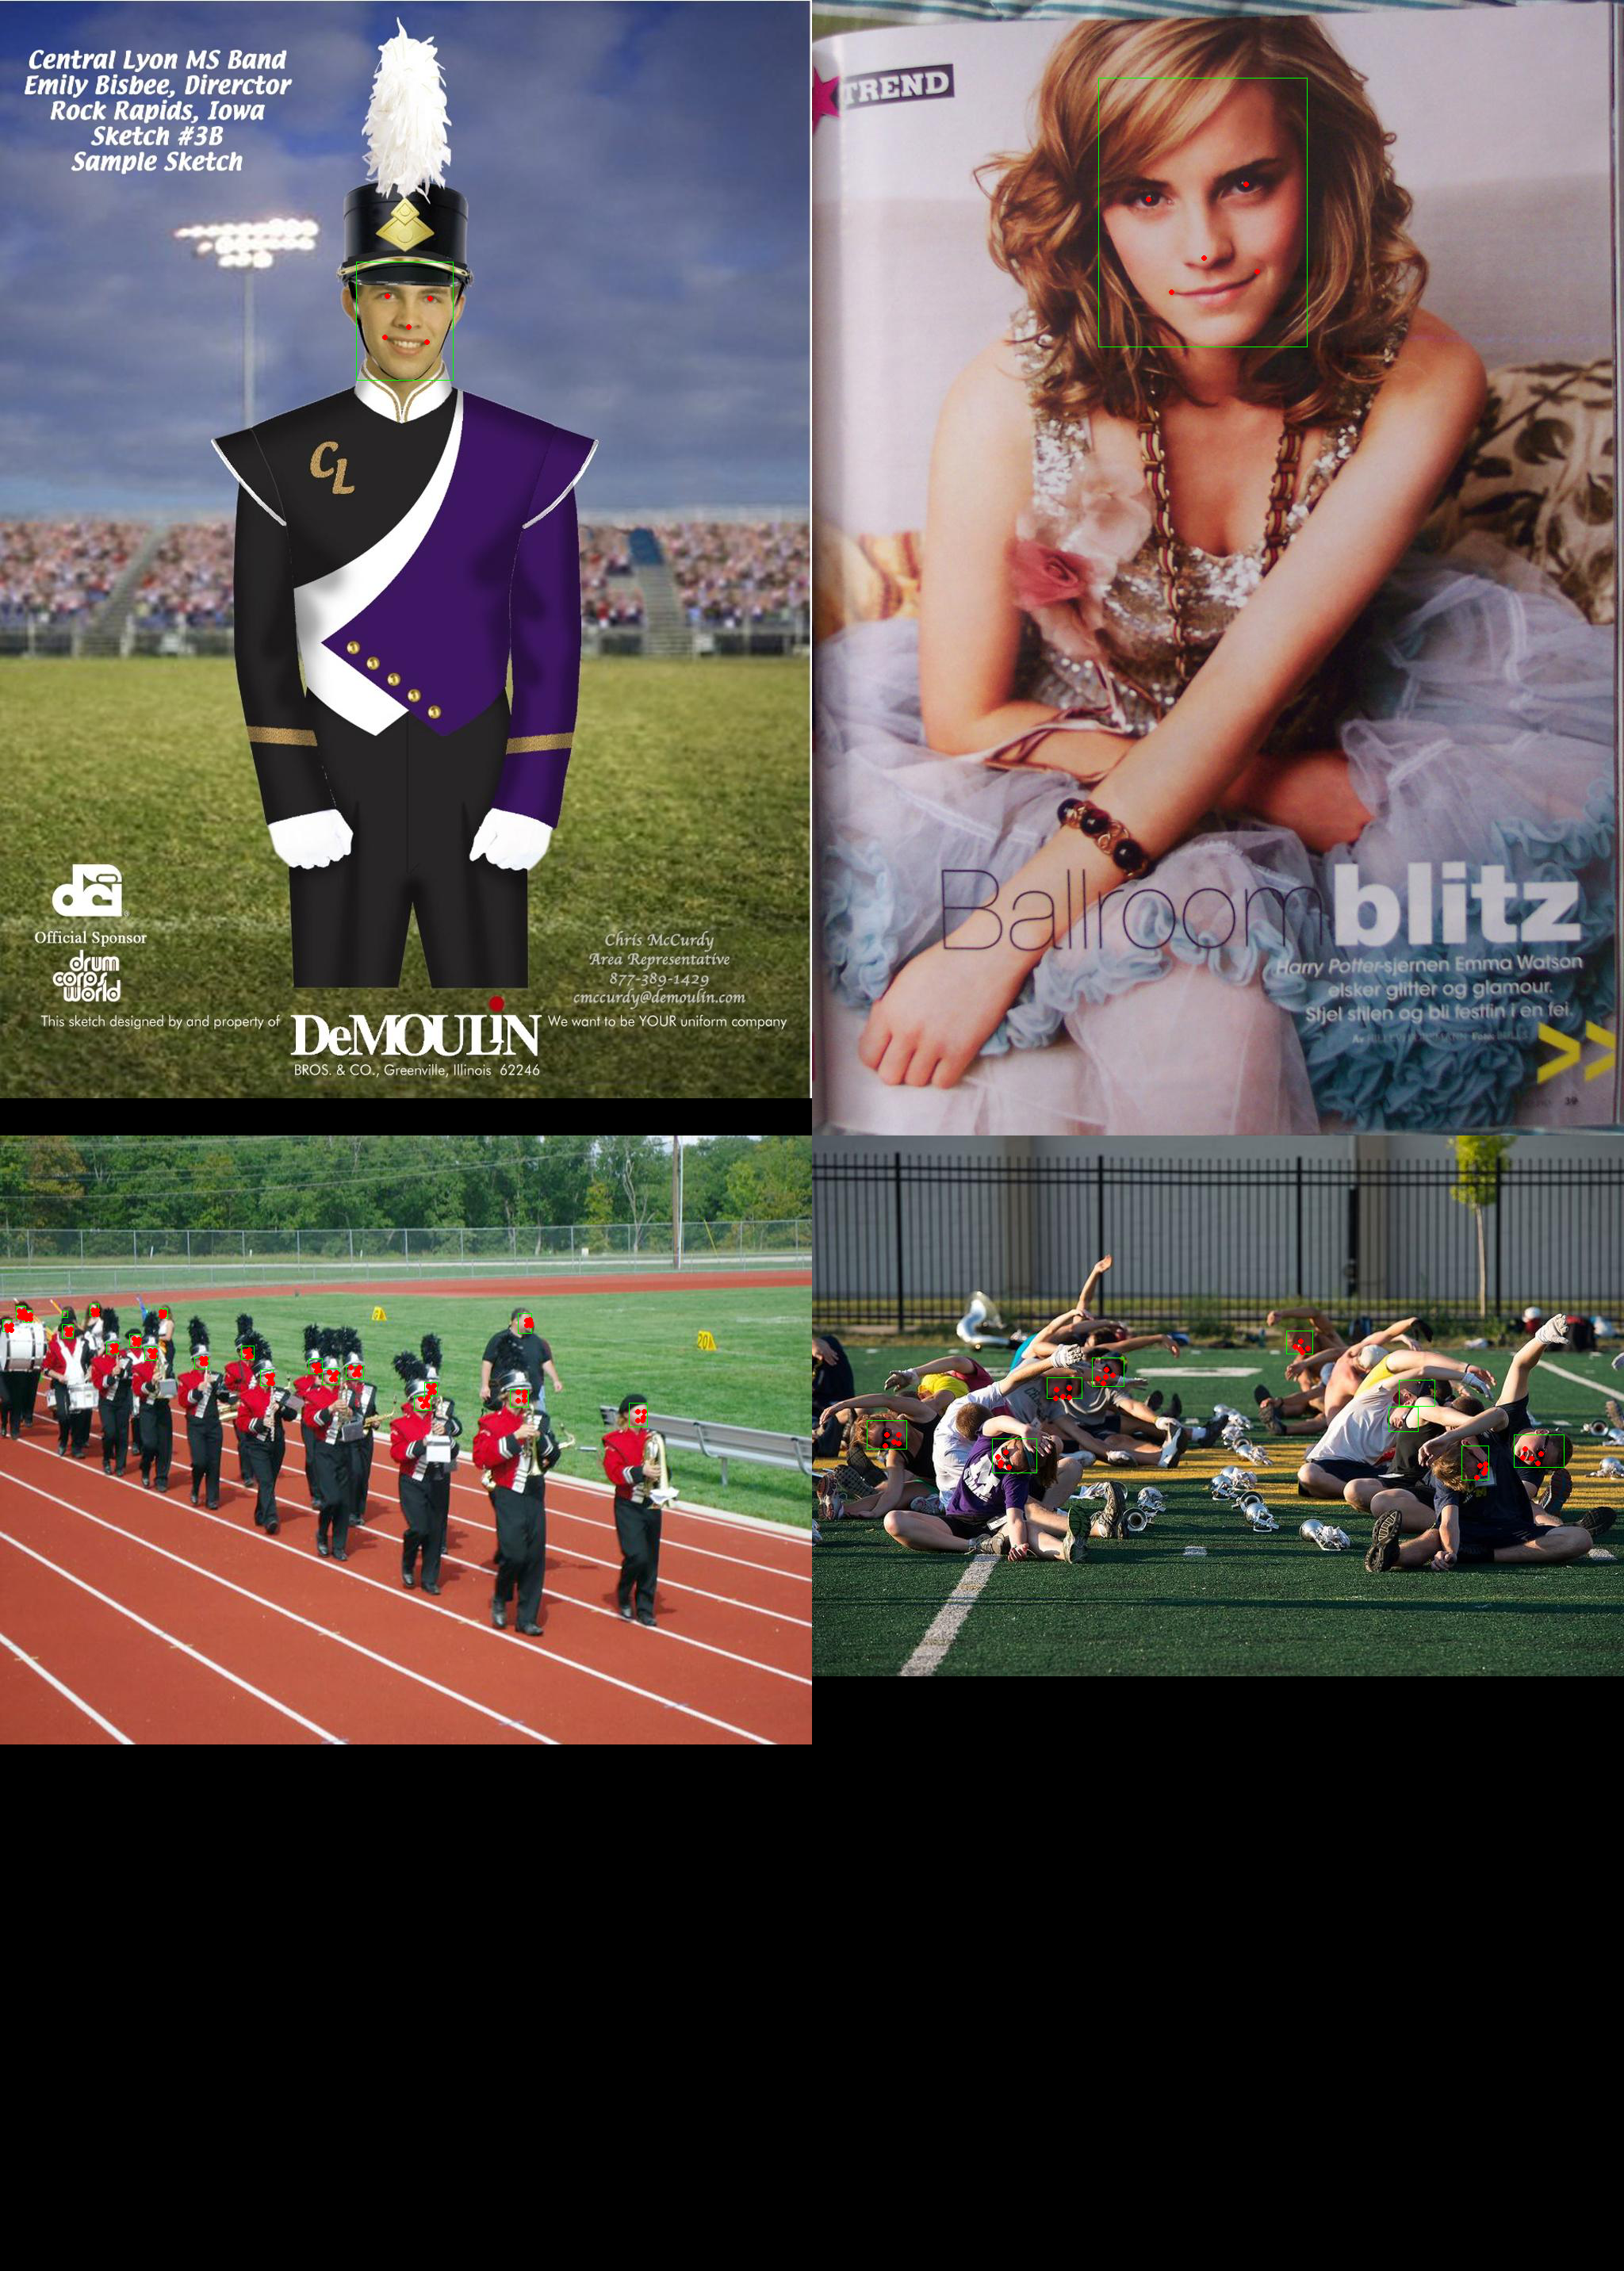
\includegraphics[width=0.8\linewidth]{img/p_all.png}
\end{figure}
\begin{figure}[H]
	\centering
	\includegraphics[width=0.8\linewidth]{img/p1.png}
\end{figure}
\begin{figure}[H]
	\centering
	\includegraphics[width=0.8\linewidth]{img/p2.png}
\end{figure}
\begin{figure}[H]
	\centering
	\includegraphics[width=0.8\linewidth]{img/p3.png}
\end{figure}
\begin{figure}[H]
	\centering
	\includegraphics[width=0.8\linewidth]{img/p4.png}
\end{figure}

\end{solution*}

\section{Initialize your detector and build up the forward path (./detector/mydetector.py).}

This face detector has 4 components: 1. ResNet 50 as Backbone. 2. Feature pyramid
network (FPN). 3. A special module named SSH. 4. Three heads for classification,
bounding box regression, and landmarks, respectively.

Note 1: Since the FPN needs a feature pyramid extracted from the backbone, you will need to use 
\begin{verbatim}
  torchvision.models._utils.IntermediateLayerGetter
\end{verbatim}

to gather these intermediate layers from backbone.

Note 2: The classification head aims to classify each anchor as positive or negative, because we
are doing face/not face here. Regression aims to regress a bounding box for each
anchor, it requires 4 degrees of freedom to do so. Landmark head aims to regress 5
landmark points, it requires 10 degrees of freedom to do so.

\subsection{Initialize backbone and gather intermediate layers, the layers to-be-gather are
defined in cfg['return layers']}

Note: cfg is "configuration" that is specified in config.py

\begin{solution*}{}
backbone = models.resnet50(pretrained=cfg['pretrain'])

self.body = \_utils.IntermediateLayerGetter(backbone,return\_layers=cfg['return\_layers'])

\end{solution*}

\subsection{Understand how we make the classification head. What is the output dimension
of the head?  And, for the binary classification, is sigmoid mathematically equivalent to softmax?  Show your proof.}

\begin{solution*}{}
1. (batch\_size, height * width * self.num\_anchors, 2)

2. Yes, for sigmoid function, it's sig(x) = 1 / (1 + exp(-x))

For Softmax Function,it's soft(x) = exp(x)/sum(exp(xi))

For binary classification, there are only two type: y==1 or y==0,
so it can be written as 

P(y = 1) = exp(x) / (exp(0) + exp(x)) = exp(x) / (1 + exp(x)) = 1 / (exp(-x) + 1), which is same as sigmoid function. 

Also, P(y = 0) =1 / (1 + exp(x)) = exp(-x) / (1 + exp(-x)) = 1- sig(x)
\end{solution*}

\subsection{Following the code of the classification head, finish the regression head and
landmarks head.}

\begin{solution*}{}

\begin{verbatim}
class BboxHead(nn.Module):
    def __init__(self, inchannels=512, num_anchors=3):
        super(BboxHead,self).__init__()
        # TODO
        self.conv1x1 = nn.Conv2d(inchannels, num_anchors * 4,
         kernel_size=(1,1),stride=1,padding=0)

\end{verbatim}

\begin{verbatim}
class LandmarkHead(nn.Module):
    def __init__(self, inchannels=512, num_anchors=3):
        super(LandmarkHead, self).__init__()
        # TODO
        self.conv1x1 = nn.Conv2d(inchannels, num_anchors * 10,
         kernel_size=(1,1),stride=1,padding=0)
\end{verbatim}
        
\end{solution*}

\subsection{Complete the forward function of your detection. The process is Input image
 $->$ gather feature maps  $->$ FPN $->$you got 3 feature pyramids  $->$ for each feature
pyramid, apply a predefined SSH module to it  $->$for each feature pyramid, apply
three heads to it.}

\begin{solution*}{}
	
	\begin{verbatim}
	# FPN
	fpn = self.fpn(out)
	
	# SSH
	feature1 = self.ssh1(fpn[0])
	feature2 = self.ssh2(fpn[1])
	feature3 = self.ssh3(fpn[2])
	features = [feature1, feature2, feature3]
		
	\end{verbatim}
	
\end{solution*}

\section{Dataloader (data/dataloader.py)}
Your dataloader feeds images, bounding boxes, and landmarks to the detector for
training.

\subsection{initialize dataloader}

\begin{verbatim}
    In __init__, load the widerface/train/label.txt, 
    and store the path of images in self.imgs_path as a list. 
    Store the annotations in self.words. The structure must be
    self.imgs_path: [path1, path2, path3]
    self.words: [[img1_anno1, img1_anno2, ...]
                [img2_anno1, img2_anno2, img2_anno3, ...]
                [img3_anno1, ...]
                    ...]
    Make sure you are storing numbers in float.
\end{verbatim}


\subsection{getitem}

Getitem is a commonly seen function in pytorch based dataloader. It aims to get/organize/process the training data from the pool prepared for each iteration.  

Read carefully:

\begin{verbatim}
    In __getitem__, complete the annotation reorganization. Each "annotation"
    should be in the following format:
    np.array(x1, y1, x2, y2, L0_x, L0_y, L1_x, L1_y, ..., L4_x, L4_y, M)
    Where (x2, y2) is the bottom-right corner of the bounding box, 
    L stands for the landmark points.
    M is an indicator showing whether landmark points are
    available, 
    Yes for 1 and No for -1. The "annotation" is in shape (1, 15)
    
\end{verbatim}


\section{Anchor(anchor.py)}
Anchor has been an important concept for detection since 2015 (Faster RCNN). 

We define "Anchor", in this homework, as "all reference boxes located in every feature point"

Understand the
code, and answer the following

\subsection{Name all hyperparameters that correspond to the number of anchors. I.e., which hyperparameters in config will affect the number of anchors?  Briefly describe their physical meanings in your words}
\begin{solution*}{}
min\_sizes: lower and upper bounds for minimum sizes for the anchors of image, the size(number of items) of this effects number of anchors.

steps: step size of placing anchors in feature map. A smaller step size results in more anchors.

image\_size: The size of the input image, used to calculate the spatial scale of the anchors. With image\_size increasing, the number of anchors also increases.
\end{solution*}
\subsection{If we enlarge the width and height of the image by x, how would the number of anchors change?}
\begin{solution*}{}
If enlarging the width and height of the image by x, the number of anchors will increase. With fixed step size, the anchor with be more with larger scale of image.
Also, the number of anchors will become \[x^2\]
\end{solution*}
\subsection{For anchors on different feature pyramids, are they the same size? Explain your
observations and explain why it is designed in such a way.}

\begin{solution*}{}
No, anchors at different scales are different.

Larger anchors works on larger and higher-resolution feature pyramids especially for smaller objects on it, and smaller anchors works on smaller and lower-resolution feature pyramids especially for larger objects on it. Size is different for different feature pyramids.

\end{solution*}


\section{Calculate the Loss}

Anchor plays a key role in anchor-based object detection for deciding which feature point
on the feature pyramid should be responsible for learning a certain ground-truth. Let’s do
a quick review:

On your multi-level feature pyramid, each pixel is a feature point. Each feature point is
mapped to one or multiple anchors depending on the detector’s setting. We use an anchor to
compare with ground-truth via “jaccard index”, i.e., Intersection over Union. If the IoU is larger
than a threshold (0.2), then the feature point corresponds to that anchor would be assign to
learn the ground-truth, the learning includes positive/negative classification, bounding box
regression, and landmark. If an anchor matches zero ground-truth, the corresponding feature
point needs to be classified as negative.

\subsection{In utils/boxutils.py, complete jaccard function.}

\subsection{Explain the following code in your words:}

In “match”, what is the following code used for?
\begin{verbatim}
best_prior_overlap, best_prior_idx = overlaps.max(1, keepdim=True)
\end{verbatim}

\begin{solution*}{}
this is used to find the best matching prior box index and value for each ground truth box based on Jaccard(IOU) result.
\end{solution*}

In “match”, what is the following code used for?

\begin{verbatim}
valid_gt_idx = best_prior_overlap[:, 0] >= 0.2
\end{verbatim}

\begin{solution*}{}
 
 Used as filter to select the one with IOU value larger than 0.2 and ignore others.
 It checks best prior box for each ground truth box.
\end{solution*}


In “match”, what is the following code used for?

\begin{verbatim}
best_truth_overlap, best_truth_idx = overlaps.max(0, keepdim=True)
\end{verbatim}
\begin{solution*}{}
this is used to find the best matching ground truth box index and value for each prior box based on Jaccard(IOU) result.
\end{solution*}


\section{NMS}
Non-maximum suppression is a must-ask question for those interviews seeking computer vision engineer positions. Prior to 2020, it is an essential component for object detection and many other
tasks. Write function of NMS in nms.py

\begin{verbatim}
input: dets: ndarray (nx5), where n is number of predictions, 
and each prediction is in (x1, y1, x2, u2, confidence)
        thres: float, which is IOU threshold.
output: list, the index of the predictions in dets, which passed NMS. 
\end{verbatim}


\section{Training}
Train your detector with 1 epoch, and plot each loss curve, the plotting step is per 20 iterations.

\begin{solution*}{}

\begin{figure}[H]
	\centering
	\includegraphics[width=0.8\linewidth]{img/loss_plot.png}
\end{figure}

\begin{figure}[H]
	\centering
	\includegraphics[width=0.8\linewidth]{img/loss_out.png}
\end{figure}

\end{solution*}

Use any methods you feel comfortable with to remove the landmark supervision. Explain your method.  And what do you expect the face detector would perform (better or worse) after the removal? Explain your answer.
\begin{solution*}{}
According to Piazza, can just remove landmark supervision from loss perspective. To do this, just delete remove landmark loss here:

loss = cfg['loc\_weight'] * loss\_l + loss\_c + loss\_landm

to:

loss = cfg['loc\_weight'] * loss\_l + loss\_c

I think it will be worse since one loss is removed and the features of landmarks are also lost. Not that much information for detection.

\end{solution*}

\section{Testing}
Load the checkpoint we provided, it is the same as yours but trained with larger batchsize and with 180 epochs. Plot the first 4 results of your detector, with confidence,
face bounding box, and landmarks.

\begin{solution*}{}
\begin{figure}[H]
	\centering
	\includegraphics[width=0.8\linewidth]{img/output_image0.jpg}
\end{figure}
\begin{figure}[H]
	\centering
	\includegraphics[width=0.8\linewidth]{img/output_image1.jpg}
\end{figure}
\begin{figure}[H]
	\centering
	\includegraphics[width=0.8\linewidth]{img/output_image2.jpg}
\end{figure}
\begin{figure}[H]
	\centering
	\includegraphics[width=0.8\linewidth]{img/output_image3.jpg}
\end{figure}
\end{solution*}


Enjoy your face detector and feel free to deploy it for your home security.

\clearpage

\textbf{Collaboration Survey} Please answer the following:

\begin{enumerate}
	\item Did you receive any help whatsoever from anyone in solving this assignment?
	\begin{checkboxes}
		\correctchoice Yes 
		\choice No
	\end{checkboxes}
	\begin{itemize}
		\item If you answered `Yes', give full details, for any type of collaboration:
		\item (e.g. “Jane Doe explained to me what is asked in Question 3.4”)
	\end{itemize}
	
	\begin{tcolorbox}[fit,height=3cm,blank, borderline={1pt}{-2pt},nobeforeafter]
		%Input your solution here.  Do not change any of the specifications of this solution box.
		1. Post question in Piazza asking question logic and debugging code.
		2. Visit OH to find how to use matrix calculation to make jaccard function faster rather than using loops.
		3. Discuss with yichuanl about what what is asking in some question like 4.3.
		
	\end{tcolorbox}
	
	\item Did you give any help whatsoever to anyone in solving this assignment?
	\begin{checkboxes}
		\correctchoice Yes
		\choice No\
	\end{checkboxes}
	\begin{itemize}
		\item If you answered `Yes', give full details, for any type of collaboration:
		\item (e.g. “I pointed Joe Smith to section 2.3 since he didn’t know how to proceed with Question 2”)
	\end{itemize}
	
	\begin{tcolorbox}[fit,height=3cm,blank, borderline={1pt}{-2pt},nobeforeafter]
		%Input your solution here.  Do not change any of the specifications of this solution box.
		Discuss with yichuanl about what what is asking in some question like 4.3.
	\end{tcolorbox}
	
	\item Note that copying code or writeup even from a collaborator or anywhere on the internet violates the \href{hhttps://www.cmu.edu/policies/student-and-student-life/academic-integrity.html}{Academic Integrity Code of Conduct}.
\end{enumerate}





\end{document}